% Template for ICASSP-2015 paper; to be used with:
% spconf.sty - ICASSP/ICIP LaTeX style file, and
% IEEEbib.bst - IEEE bibliography style file.
% --------------------------------------------------------------------------
\documentclass{article}
\usepackage{spconf,amsmath,graphicx}
\usepackage{hyperref}
\usepackage{amsmath}
\usepackage{amssymb}
\usepackage{graphicx}
\usepackage{listings}
\usepackage{color}
\usepackage{hyperref}
\usepackage{pxfonts}
\usepackage[]{mcode}

% Example definitions.
% --------------------
\def\x{{\mathbf x}}
\def\L{{\cal L}}

% Title.
% ------
\title{3D AUDIO RECONSTRUCTION AND SPEAKER RECOGNITION USING SUPERVISED LEARNING METHODS BASED ON VOICE AND VISUAL CUES}
%
% Single address.
% ---------------
\name{Ramin Anushiravani$^{\dag}$, Marcell Vazquez-Chanlatte$^{*\ddag}$, Faraz Faghri$^{*}$}
\address{University of Illinois at Urbana-Champaign\\$^{\dag}$Dept. of Electrical and Computer Engineering \\ $^{*}$Dept. of Computer Science \\ $^{\ddag}$Dept. of Physics}

\begin{document}
%\ninept
%
\maketitle
%
\begin{abstract}
In this paper we present a creative approach to reconstruct 3D audio for multiple sources from a single channel input by detecting and tracking visual cues using supervised learning methods. We also discuss a similar approach for improving speaker's classification from a video stream by employing both facial and speech likelihoods, in another word performing Multimodal Speaker Recognition in a video stream. 
\end{abstract}
%
\begin{keywords}
3D audio, speaker classification, visual cues, supervised learning, Multimodal Speaker Recognition
\end{keywords}
%
\section{Introduction}
\label{sec:intro}

Spatial audio and speaker classifications, both have important applications in video conferencing and entertainment. With spatial audio, one can listen to music and feel the depth and the directionality of the sound using headphones or crosstalk canceller speakers [1]. Imagine hearing a tank approaching you from the living room when playing high-end resolution video games. 3D audio is yet to be able achieve these ambitious goals, though it can still create a more realistic sound fields than surround sound. 3D audio is normally recorded through binaural microphones mounted on a Kemar [2]. One can also reconstruct 3D audio using Head Related Transfer Function by forming beams at every direction using microphone arrays [3]. These techniques require precise calibration and are not very accurate in real environments due to noise and reverberation. Most importantly, if a video was not recorded using microphone arrays or binaural microphones, it is too difficult, if not impossible, to recover spatial audio. That is why we purpose a method by using the contents in the video, the visual cues, to help reconstructing 3D audio. 
\\
The other goal of this project is to perform multimodal speaker recognition using facial and speech likelihoods by first learning different features from a training video using a user friendly calibration procedure discussed in this paper. In section II, we talk about the general flow of the algorithm for reconstructing 3D audio and speaker recognition algorithms. In section III, face detection, classification, and tracking are discussed in details. In section IV, voice activity detection (VAD) and speech classification algorithms are explained thoroughly. In section V, we go over the results for 3D audio reconstruction and multimodal speaker recognition. And finally, in section VI, we suggest future possibilities for our project in other systems and applications. 


\section{General Flow}
\label{ssec:subhead}
In this section, the basic procedure for reconstructing 3D audio and multimodal speaker recognition are discussed.
\subsection{3D Audio Reconstruction}
One can reconstruct a 3D audio by simply convolving a mono sound with the spatial response corresponding to a desired location in space. These impulse responses can be captured by recording a maximum length sequence (MLS) at listener's ears at different angles. We can then extract corresponding impulse responses by cross-correlating the recorded MLS with the original MLS as shown in equation 1. These spatial responses are also called head Related Impulse Response (hrir). 
\begin{subequations}
\begin{gather}
index = argmax({C_{(MLS_{recorded},MLS_{original})}})\\
hrir = C_{(MLS_{recorded},MLS_{original})}(index-L:index+L)\\
3D_{audio} = signal_{mono} * hrir
\end{gather}
\end{subequations}
Where $L$ is half the impulse response desired length. This number is usually about 128 samples, but it can differ based on the recording room, e.g. such the early reflection sample index and $C_{xy}$ represents the cross-correlation between $x$ and $y$. In this project we used MIT HRTF database for reconstructing spatial audio [4]. \\ 

In order to avoid clicking sounds when reconstructing 3D audio and also for simplicity, we did the reconstruction in frequency domain. In short, one must first find the short time Fourier transform of the signal and then multiplied that by the desired zero-padded HRTF and take inverse STFT to recover the time domain signal back, as shown in figure 1. 

\begin{figure}[htb]
\begin{minipage}[b]{0.88\linewidth}
\centering
\centerline{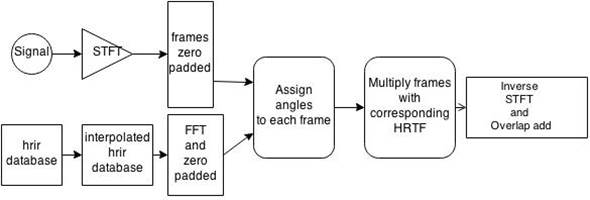
\includegraphics[width=8.0cm]{3d.jpg}}
\end{minipage}
\caption{3D Audio Reconstruction}
\label{fig:res}
\end{figure}
\centerline{}

We made a few assumptions to make this project doable in our limited timeline. \\ \\
{\it 1- This algorithm is only able to spatialize speech based on a speaker's face.
\\ 2- There are at most two speakers in the video. 
\\ 3- At least one of the two speakers in the room is in the training database.
\\ 4- There are no sudden movements in the video stream.}\\ \\

Most of this assumption can be relaxed even further, some which are discussed in section VI. For simplicity, we used the following video clip for testing our applications. \\
We recorded a video clip of two people sitting on left and right of a video frame having a conversation, as shown in figure 2. We also purpose a calibration procedure that require some user interference for training facial and speech database from each user.

\begin{figure}[htb]
\begin{minipage}[b]{0.88\linewidth}
\centering
\centerline{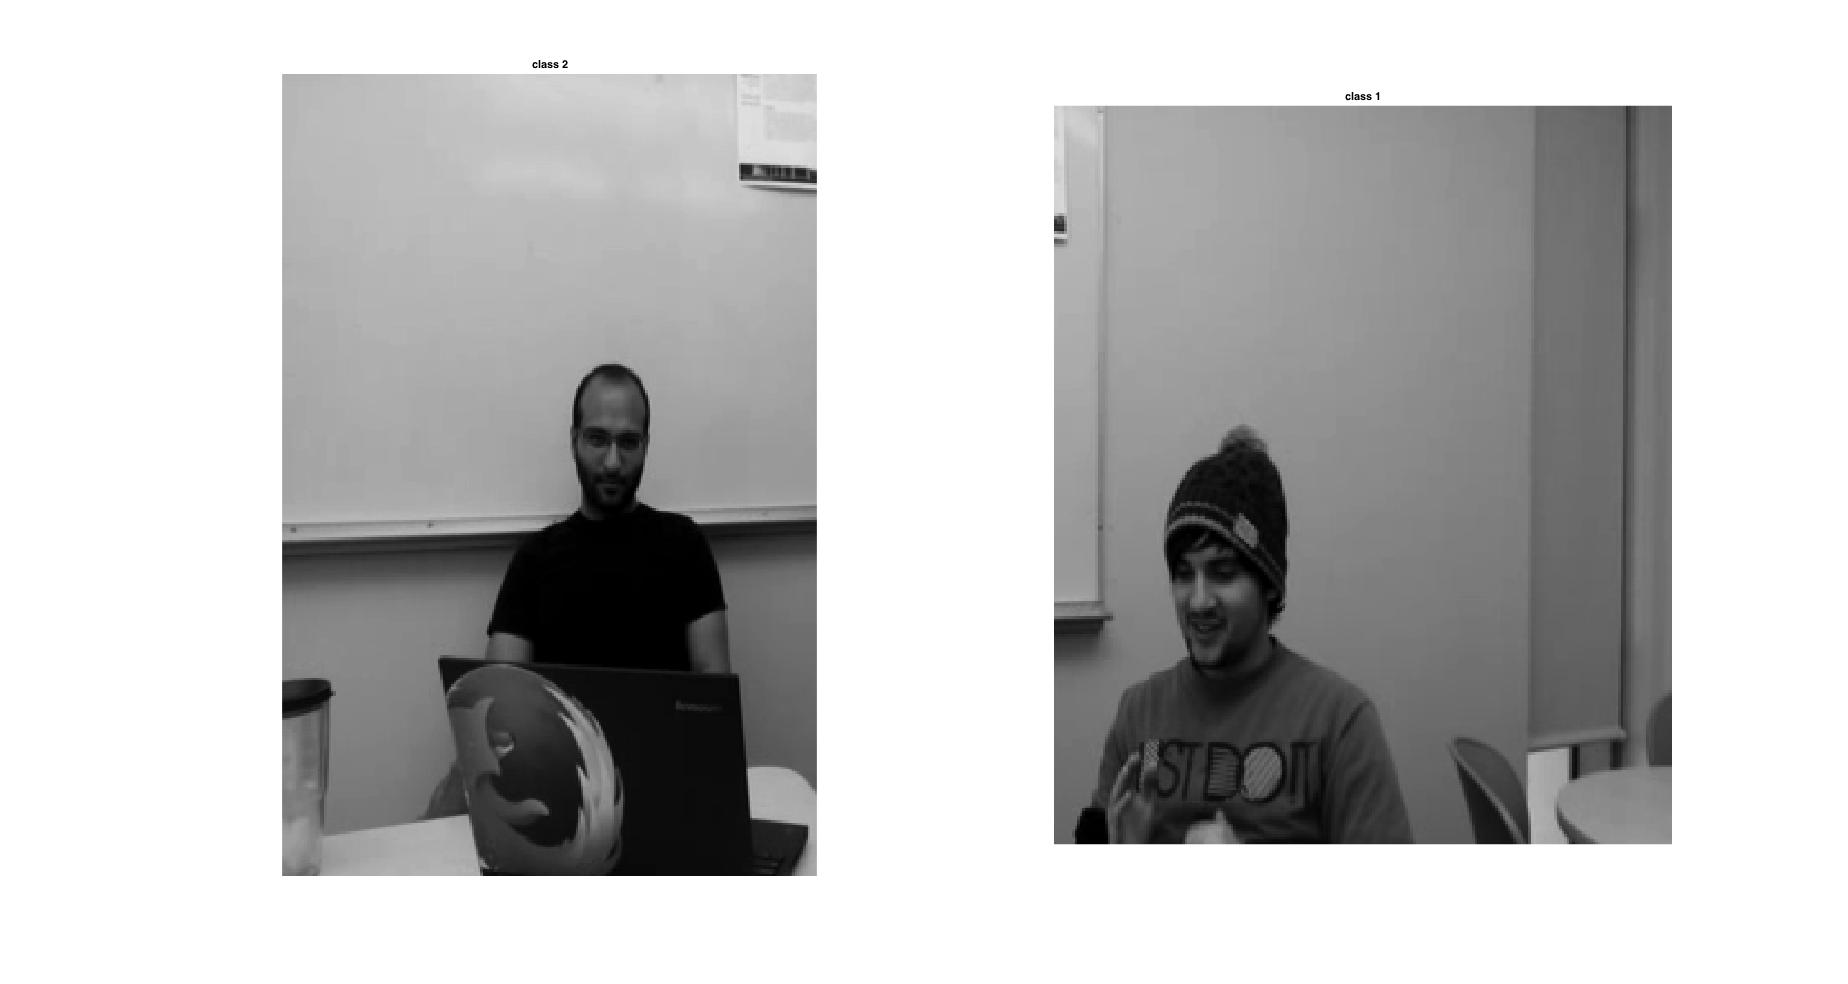
\includegraphics[width=8.0cm]{faraz_marcell.jpg}}
\end{minipage}
\caption{Recording of two people having a conversation}
\label{fig:res}
\end{figure}
\centerline{}

The calibration procedure is as follows, \\
\\
{\it Calibration \\ \\
Each user is asked to, \\
1- Clap hands and wave to the camera. \\
2- Speak for about a minutes while facing the camera. \\ }\\
This calibration procedure is repeated until another clap sound is detected, which means there is another user whose database needs to be collected as well. This calibration procedure helps us particularly in labeling the training database. \\

This is summarized in figure 3 below. 
\begin{figure}[htb]
\begin{minipage}[b]{0.88\linewidth}
\centering
\centerline{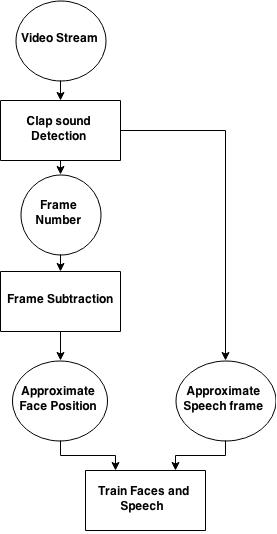
\includegraphics[width=4.0cm]{calibration.jpg}}
\end{minipage}
\caption{Calibration}
\label{fig:res}
\end{figure}
\centerline{}

After collecting a training database, we proceed making classifier which is discussed in more details in section III and IV. \\ The procedure for reconstructing a 3D audio is as follows, \\

{\it 3D Audio Reconstruction \\ \\
1- Detect faces in the video stream for each frame and classify them to one in the database. \\
2- Map the position of each face to a meaningful HRTF angle in each frame. \\ 
3- Detect whether there is speech in a frame or not. \\
4- Label the frames with speech from step 4 with their corresponding class label in the database. \\
5- Use speech classification results to assign the speech from step 4 to the point find from step 2. That is, given a speech signal, find corresponding face location. \\
6- Pick corresponding HRTFs from step 5 for each frame. \\
7- Reconstruct 3D audio as shown in figure 1. }

\subsection{Speaker Recognition}

Consider the same video from section 2.1. We would like to be able to identify each user using their facial and speech features. If the speaker is not talking, then the recognition system should put more weight towards the facial classifier. If the speaker's face cannot be detected, then the classification algorithm only uses the speech classifier. If both face and speech are available, then the classification algorithm will use both with some weighting on each model to determine and identify each user for maximizing the user recognition likelihood given the training database. 
\begin{align*}
P(user) = P(face|model)^{W_i}P(face \ model)+...\\P(speech|model)^{W_{max}-W_i}P(speech \ model)
\ \ \ \ \ \ \ \ \ \ \ \ \ \ \ \ \ \ \ \ \ \ \ \ (2)
\end{align*}
The prior probabilities in equation 2 are assumed to be equally probable, however, in practice for better accuracy they need to be estimated more carefully given the environment and the recording equipment. \\
Steps 1 through 4 in {\it 3D Audio Reconstruction} are also performed when doing speaker recognition. After having a training database for faces and speech, we then do the following, 
\centerline{}
{\it Multimodal Speaker Recognition \\ \\
5- Find the likelihood of each user's face given the face model in each frame analysis. \\
6- Find the likelihood of each user's speech given the speech model in each frame analysis.\\ 
7- Plug the values from step 5 and 6 in equation 2. \\ 
8- Determine the value of equation 2 for $w=1, 2..., 10$. \\
9- Find $w$ such that, $argmax_w(P(user))$. }\\
\\ Higher $w$'s shows that the face classification results was better than speech classification results, and so we should put more weight on the facial classifier. This could be due to the quality of the training set, or just the fact that the face classifier works better than the speech classifier. As an example, one way of choosing $w$ is measure the SNR of the signal, and put more weight on the speech classifier when the SNR is higher. With figure 4 summarizing the general flow of this project, we conclude section II. 
\begin{figure}[htb]
\begin{minipage}[b]{0.98\linewidth}
\centering
\centerline{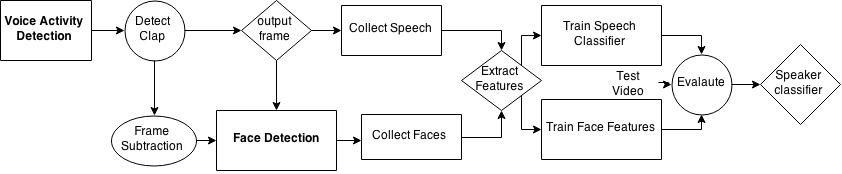
\includegraphics[width=9.0cm]{project_598ps.jpg}}
\end{minipage}
\caption{Speaker Classification}
\label{fig:res}
\end{figure}

\section{FACE DETECTION, CLASSIFICATION AND TRACKING}
In this section, we discuss the details of detecting faces in a video stream, training facial features, and tracking faces throughout the video frames. 
\subsection{Face Detection}
The first step in detecting faces is preprocessing every frame. In most image processing application, preprocessing is done to assure better quality results. For this project the preprocessing steps are as follows, \\ \\
{\it 1- Resize the video frames to smaller dimensions so we can detect faces faster.\\
2- Map the RGB color to gray colormap to simplify the computation. \\
3- Apply histogram equalization to each frame to make sure the contrast is evenly spread out throughout the whole pixels.}\\ \\
We then setup Matlab's vision library for face detection [5]. Since some detected faces are going to be small, we defined a threshold that would disregard any faces smaller than a certain number of pixels. This would create a precise training database. We then resize and vectorised all detected faces into a matrix for each user (face database). This is summarized in figure 5.
\begin{figure}[htb]
\begin{minipage}[b]{0.88\linewidth}
\centering
\centerline{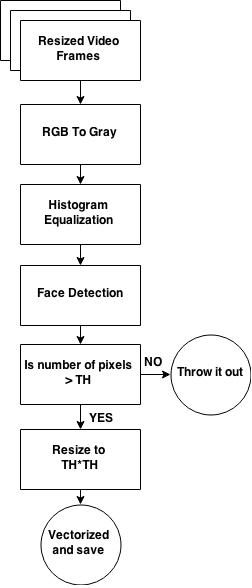
\includegraphics[width=3.0cm]{face_detection.jpg}}
\end{minipage}
\caption{Face Detection}
\label{fig:res}
\end{figure}

Note that if there is more than one user in the room, we need to be able to identify the approximate location of each so we can label them. This is why we defined the calibration procedure in section II. We first attempted to find this location by detecting mouth movement, however, due to resizing; the resolution was not high enough to detect lips movement. For simplicity, we ask our users to clap and wave to the camera, since it is easier to detect a bigger area of a motion. We simply use frame subtraction to identify the pixels that corresponds to higher variance. The clap sound detection from previous section will tell us the approximate frame number for the clap motion in the video, so the area of search is only a few frames. 
\begin{gather*}
sub_{frame} = (frame_i - mean(frame_{1:i-1}))^2 \\ 
[i_{max}, j_{max}] = max(sub_{i=1:n,j=1:m})
\end{gather*}

Where $n$ and $m$ are the number of pixels in the vertical and horizontal axis. We don't care for the exact position of those high variant pixels, we only need an approximation of which part of the frame that specific user is located at, e.g. left, right, up, down. The resulting pictures for frame subtraction, division and face detection is shown in figure 6.
\begin{figure}[htb]
\begin{minipage}[b]{0.88\linewidth}
\centerline{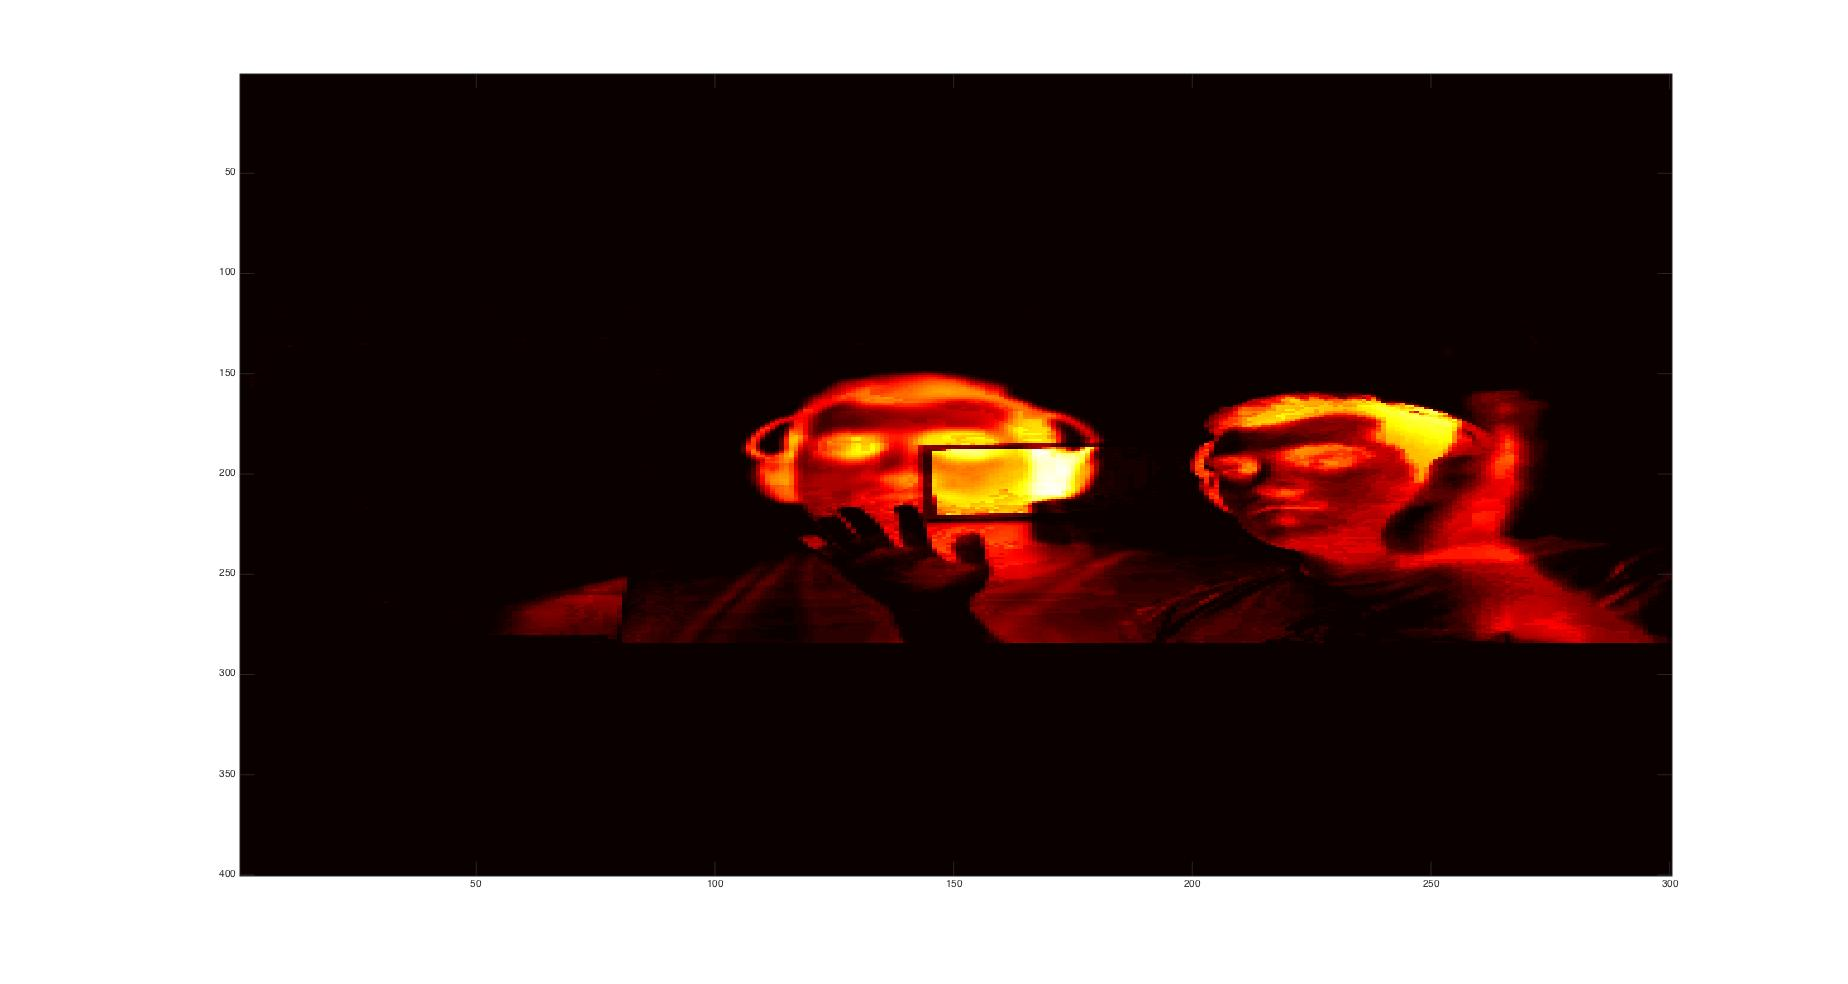
\includegraphics[width=5.60cm]{clap_motion.jpg}}
\centerline{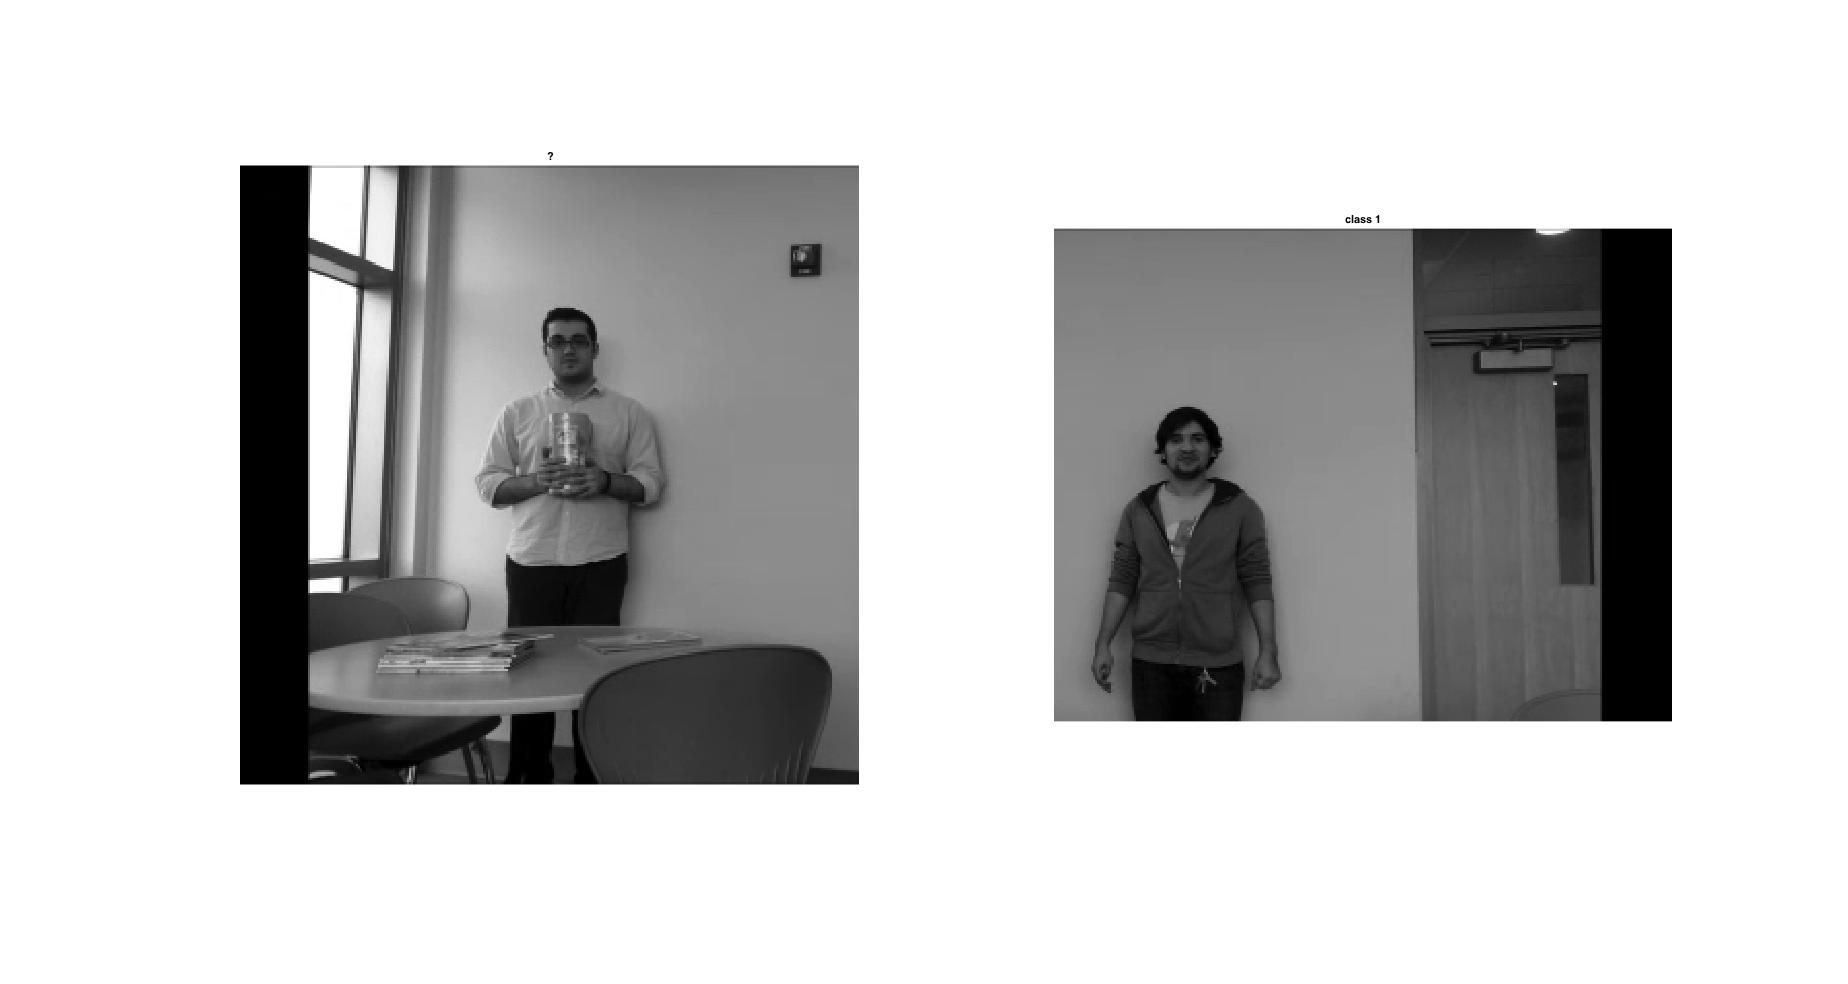
\includegraphics[width=6.60cm]{3d_audio_tracking_1.jpg}}
\centerline{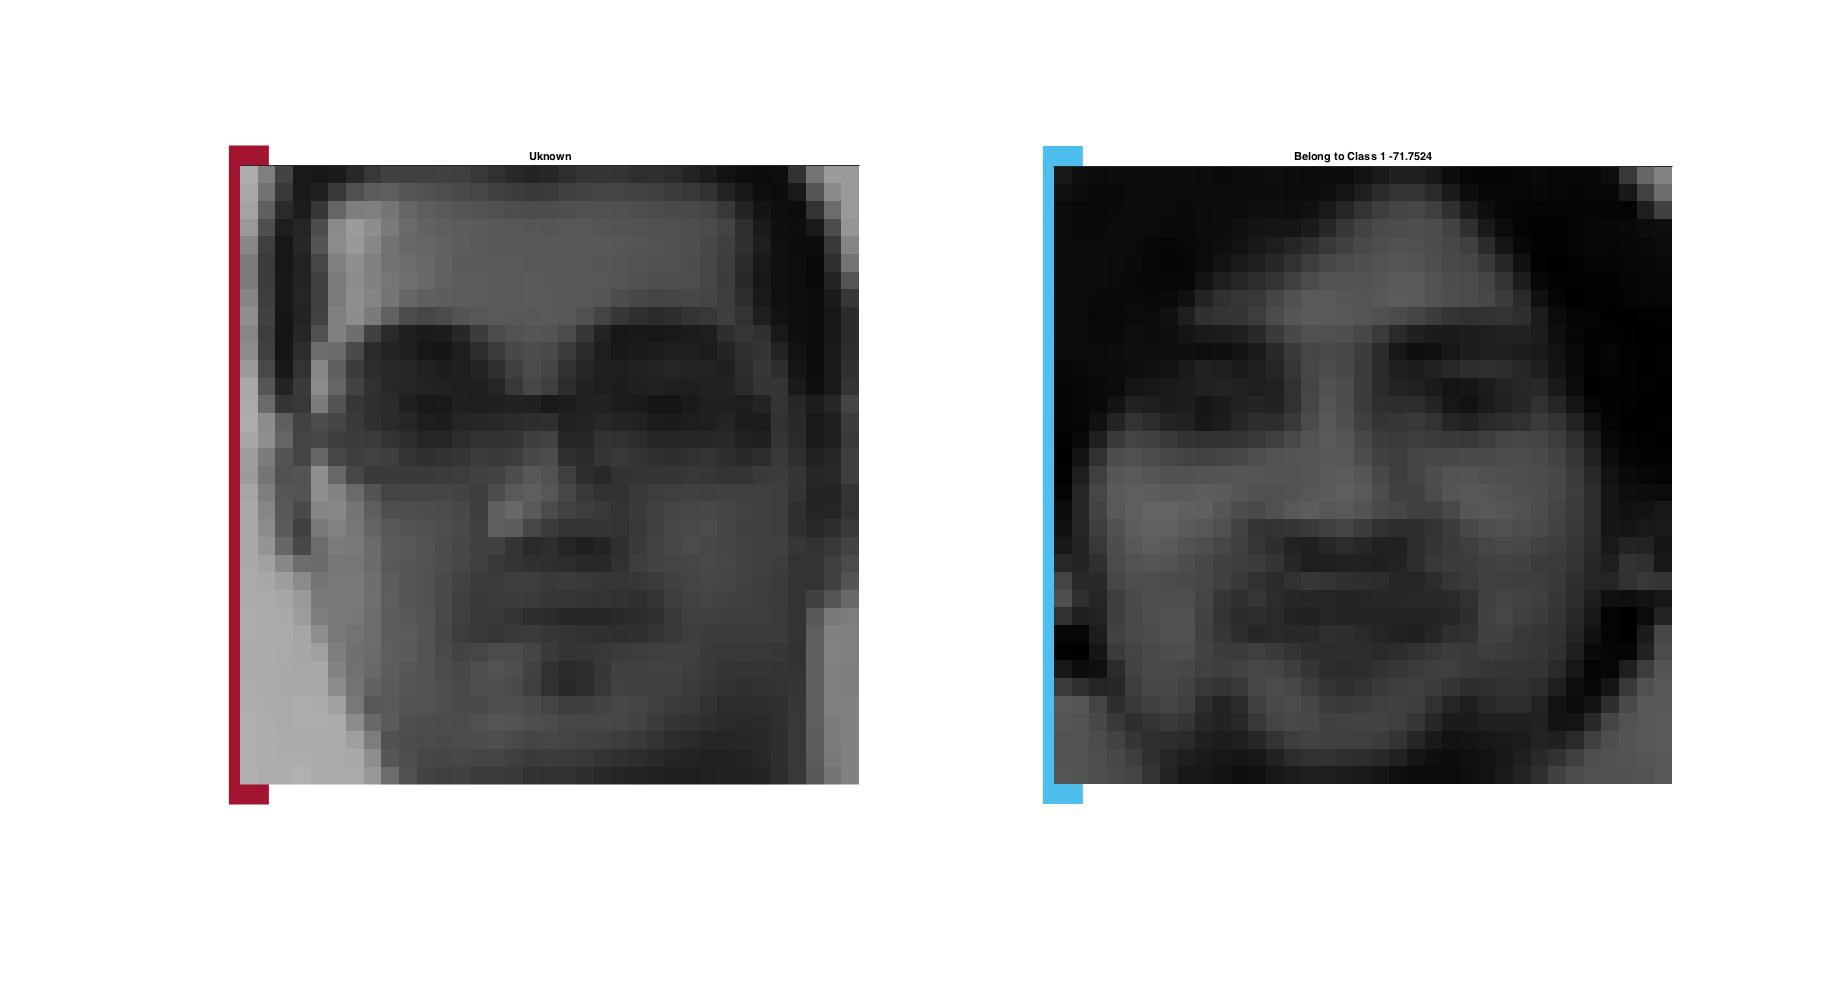
\includegraphics[width=3.0cm]{3d_audio_tracking_2.jpg}}
\end{minipage}
\caption{Frame subtraction and division into two partitions for labeling each class}
\label{fig:res}
\end{figure}

\subsection{Face Classification}
Now that we have a database of faces for each user, we need to train each database. We used Gaussian Mixture Models for training the facial database. Since the dimensions of the training database are fairly large, we first lower the dimensionality of the database using PCA to 36 and then use a 5 order GMM to fit it to the model. Dimensionality reduction is also important when training a database with a GMM, since in high dimensions; GMM might not able to estimate the covariance matrix. Face training is summarized below. 
\begin{subequations}
\begin{gather}
Train = \{train_{user1}, train_{user2}\} \\ 
Pt = PCA(train,number\ of\ eigenvector) \\ 
Gpt = GMM(pt,dimensions)
\end{gather}
\end{subequations}

\centerline{}
The eigen faces from the PCA is shown in figure 7. 
\begin{figure}[htb]
\begin{minipage}[b]{0.98\linewidth}
\centerline{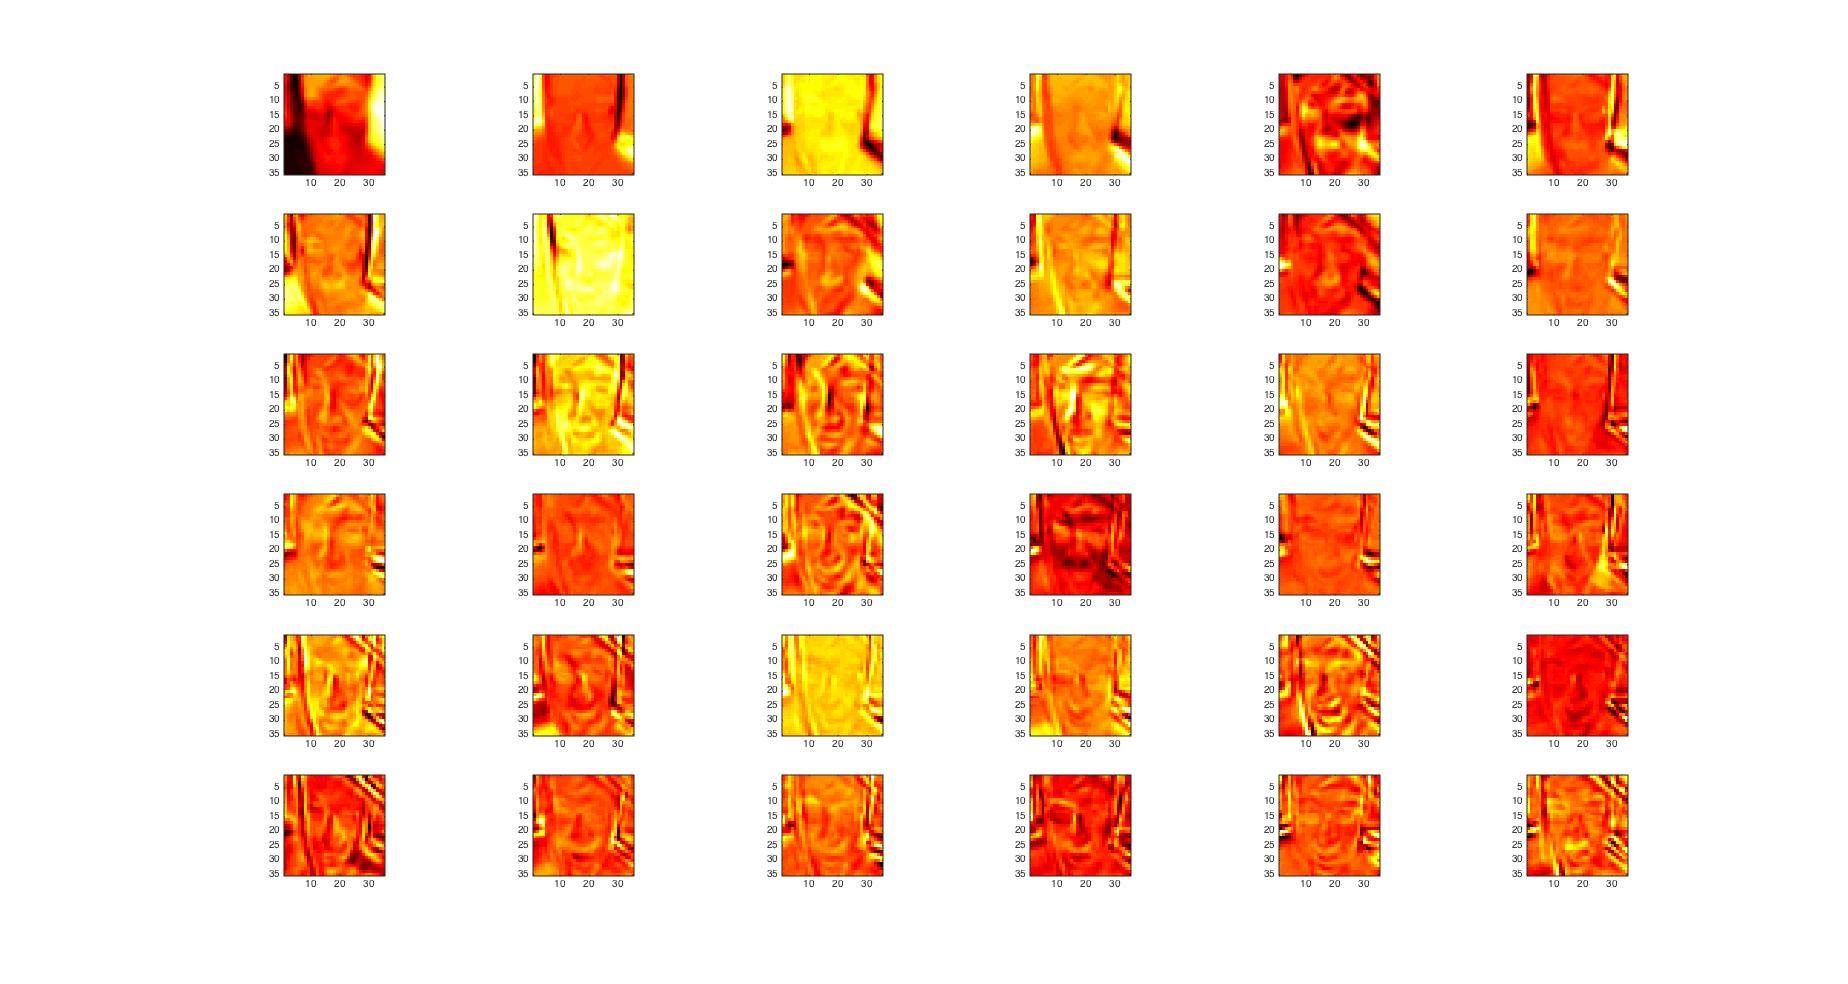
\includegraphics[width=8.60cm]{eigen_face.jpg}}
\end{minipage}
\caption{Eigen faces for class 1}
\label{fig:res}
\end{figure}
Having the GMM model for each database, one can then easily find the probability of each face given each model by calculating the log likelihood of the testing data that is projected to PCA space in equation 2.b, given the mean and the variance find in equation 2.c. This is shown in equation 3. 
\begin{align}
f(test|\mu,\sigma) = \frac{1}{test\ \sigma\sqrt{w\pi}}e^\frac{ln(x-\mu)^2}{2\sigma^2}
\end{align}
In figure 8, the scatter plot each class using the first two highest eigenvector from the PCA matrix is shown. As you can see the two classes are linearly separable, so we should be able to get high accuracy from our classifier. 
\begin{figure}[htb]
\begin{minipage}[b]{0.88\linewidth}
\centerline{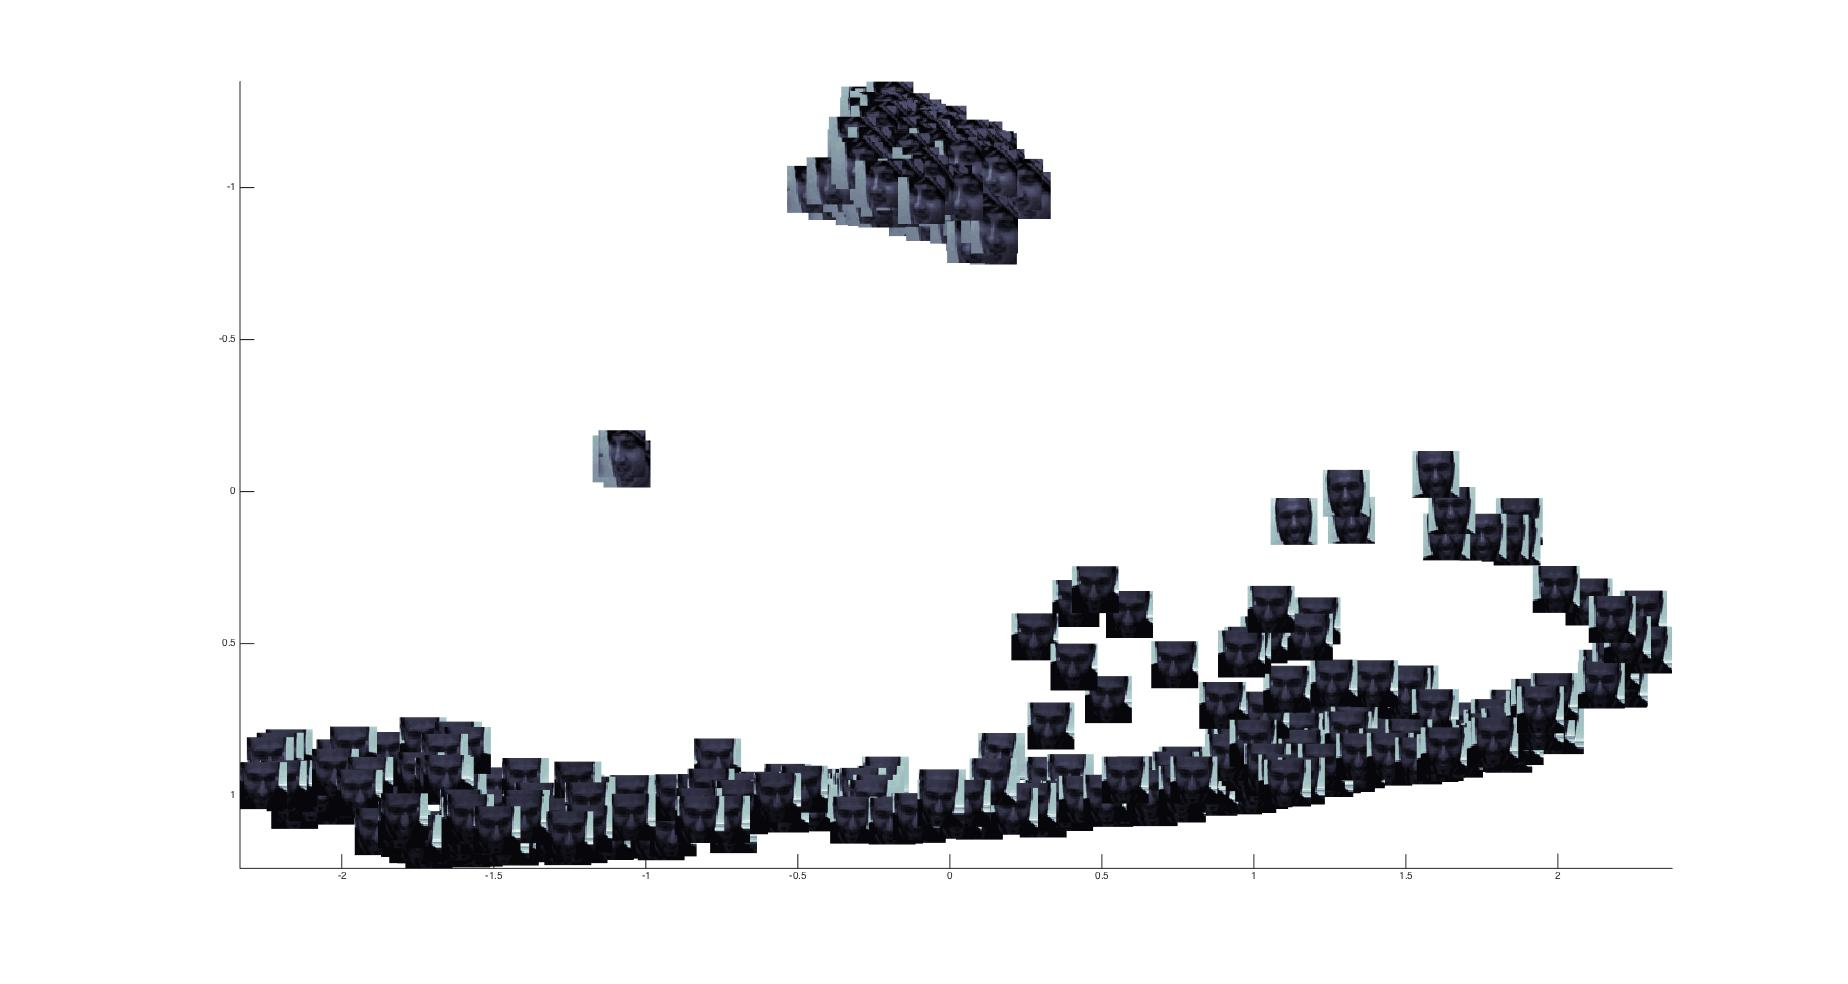
\includegraphics[width=8.60cm]{scatter_face.jpg}}
\end{minipage}
\caption{2 Dim PCA Face Features}
\label{fig:res}
\end{figure}
We left $10\%$ of our training database for testing and trained the remaining $90\%$. The result of our facial classifier is tabulated below. \\

\begin{center}
\begin{tabular}{ | l|c | r| }
\hline
Class 1 & $95\%$ \\ \hline
Class 2 & $100\%$ \\ \hline
\end{tabular}
\end{center}\centerline{Table 1: Face Classification Accuracy}

\centerline{}
As expected we have high accuracies, since the two classes were shown to be linearly separable in 2 dimensions. 
\subsection{Face Tracking} 
Matlab's face detection function draw a rectangle around the detected faces. We extracted the coordinates for that rectangle and use the center of the rectangle as the position of the detected user. Such tracking algorithm usually does give good results due to face detection inaccuracy. Since we do not need to know the exact position of the user at each frame, we can compensate for this flaw by applying moving average to the tracking results as well as fitting a polynomial to it (in this case a polynomial of order 10 and moving average of 25 frames length). If the sources were stationary we can use a longer moving average for smoothing the results. The result of such process is shown in figure 9. 
\begin{figure}[htb]
\begin{minipage}[b]{0.88\linewidth}
\centerline{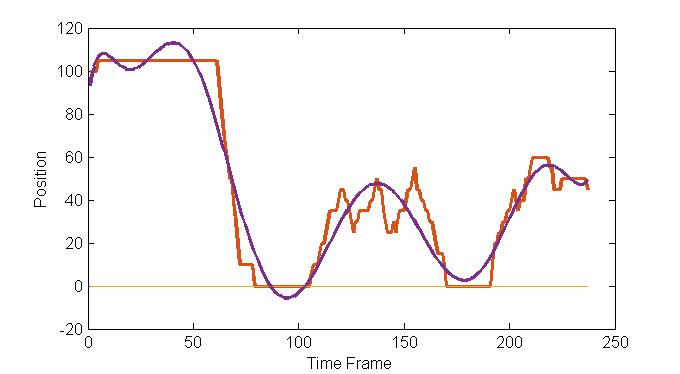
\includegraphics[width=6.8cm]{tracking_results.jpg}}
\end{minipage}
\caption{Tracking Results}
\label{fig:res}
\end{figure}
The $x-axis$ corresponds to the time frame, and the $y-axis$ is the approximated $x-position$ of the detected face. We only look at things in the azimuth, since the 3D audio does not sound very good for elevation angles. \\
In general, for recreating sptial audio for $n$ people, we need at least $n-1$ training databases. As discussed in section 2.1 we assumed that we only have up to 2 users in a video frame. Therefore, if we have the training dataset for one of the users, we can classify one in the databse with a lable and define a threshold for the other user; so we can label him/her as unknown class. This threshold is defined as following, 
\begin{align*}
if \ P(face|model)<TH \\ then\ \ \ 
Face_{label} : unknown
\end{align*}
The tracking result of having one unknown and one known user in a frame video shown in figure 6 is shown in figure 10. 
\begin{figure}[htb]
\begin{minipage}[b]{0.88\linewidth}
\centerline{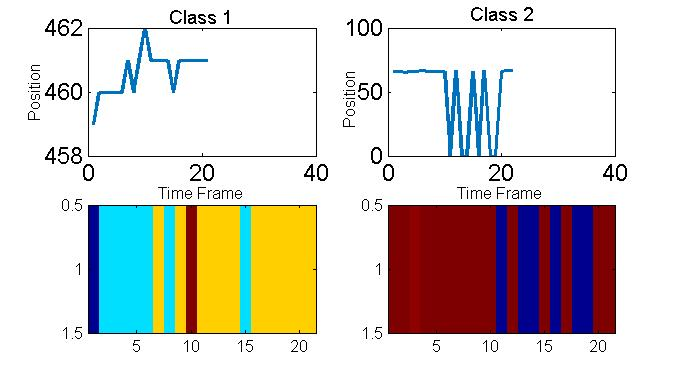
\includegraphics[width=8.8cm]{3d_audio_tracking_3.jpg}}
\end{minipage}
\caption{Tracking results for two users, one labeled, and one unknown}
\label{fig:res}
\end{figure}
As you can see, each source is correctly detected at opposite edge of each video frame. The spikes in these graphs are mainly for two reasons, 1- slight head movement and 2- Face detection errors. As mentioned earlier, the first problem can be ease out by using moving average and the second problem by fitting a polynomial to the database as seen in figure 9. The spectrogram shown in figure 10 is also the tracking results; we mainly use it since it is clearer when visualizing the tracking over video frames. 
\section{VOICE ACTIVITY DETECTION AND CLASSIFICATION}
\subsection{Voice Activity Detection}
In order to have a good speech recognition system, we remove the non-speech components (silences) from the desired signal. This way the only signal that we have in our training database is speech. As mentioned earlier in section 2, the calibration procedure help labeling the speech signals, so we already know the approximate time interval in the signal for each user. \\
In order to do VAD, we developed a supervised method by training speech and non-speech signals. We used log spectral coefficients (LSC) and Mel frequency cepstral coefficients (MFCC) as speech features. The classification results for four different classifiers are listed in table 2. \\
\begin{center}
\begin{tabular}{ | l|c | r| }
\hline
Classifier & LSC & MFCC \\ \hline
Linear SVM & $99.9\%$ & $99.9\%$ \\ \hline
Gaussian Naive Bayes & $99.9\%$ & $ 99.9\%$ \\ \hline
20-Nearest Neighbor & $99.9\%$ & $ 99.9\%$ \\ \hline
\end{tabular}
\end{center}\centerline{Table 2: VAD Accuracy}
\centerline{}
As you can see the results from each classifier is near perfect. We chose linear SVM for further processing, due to its simplicity. 
\\ After removing non-speech components from the signal, we create a database of each user's speech using the calibration procedure mentioned in section 2.1. We now train each database separately like we did for faces in section III. 
\subsection{Voice Classification}
10\% of the data was separated for testing and the remaining 90\% for training speech models for each class. When taking the STFT of the signal, we use frame analysis that are as long as the camera recorder frame rate per second (25 fps in our case), with no overlap, using rectangular windows. This is because we would like to be able assign the face location to easily assign each speech frame. We also tried averaging over a number of frames to speed up the process.\\
After extracting LSC and MFCC features from each class, we project them to a lower dimensional space using PCA, as we did when training a face database for each user in section 3. \\
The corresponding LCS and MFCC features are shown for a 2 dimensional space in figure 11 for non-speech signals, class 1 and class 2 speech signals.
As you can see non-speech and speech classes are linearly separable for LSC features and non-linearly separable for MFCC features. However, neither of the speech classes are separable in 2 dimensions for either features. We can only hope that using more PCA dimensions will help separating the two classes in higher dimensions. 
\ The procedure for classifying speech is summarized in figure 12. The resulting classification results are shown in table 2 below. As you can see Ada-Boost has the highest classification accuracy among all.
\begin{center}
\begin{tabular}{ | l|c | r| }
\hline
Classifier & LSC & MFCC \\ \hline
Linear SVM & $83.0\%$ & $85.3\%$ \\ \hline
Gaussian Naive Bayes & $82.4\%$ & $80.2\%$ \\ \hline
20-Nearest Neighbor & $84.9\%$ & $ 86.7\%$ \\ \hline
Ada-Boost & $91.2\%$ & $ 90.3\%$ \\ \hline
GMM & $83.5\%$ & $---$\\ \hline
\end{tabular}
\end{center}\centerline{Table 2: VAD Accuracy}

\begin{figure}[htb]
\begin{minipage}[b]{0.88\linewidth}
\centerline{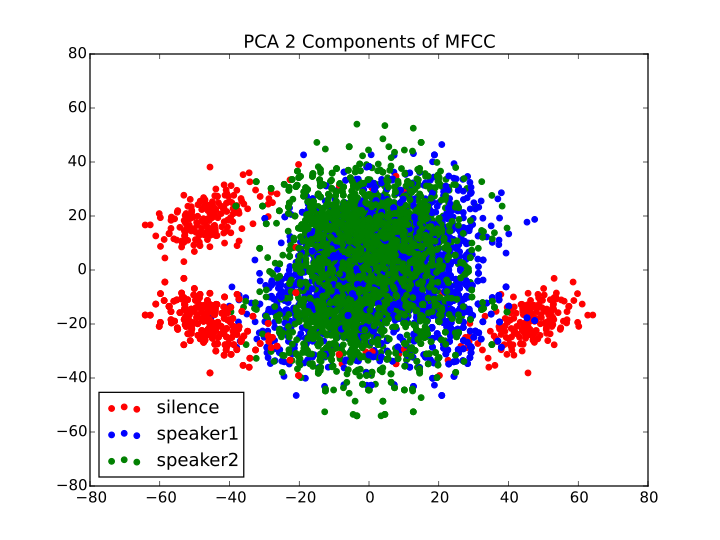
\includegraphics[width=6.6cm]{mfcc_2pca.png}}
\centerline{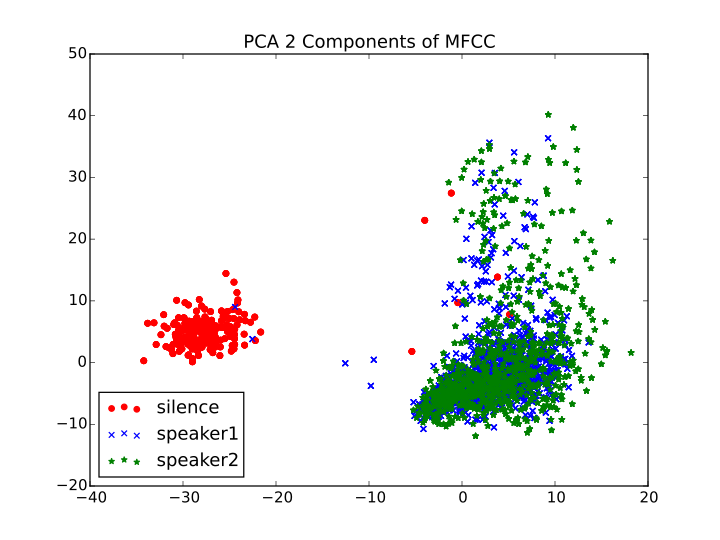
\includegraphics[width=6.6cm]{spectral_log_2pca.png}}
\end{minipage}
\caption{MFCC (top) and LSC features (bottom) for three classes}
\label{fig:res}
\end{figure}

\begin{figure}[htb]
\begin{minipage}[b]{0.88\linewidth}
\centerline{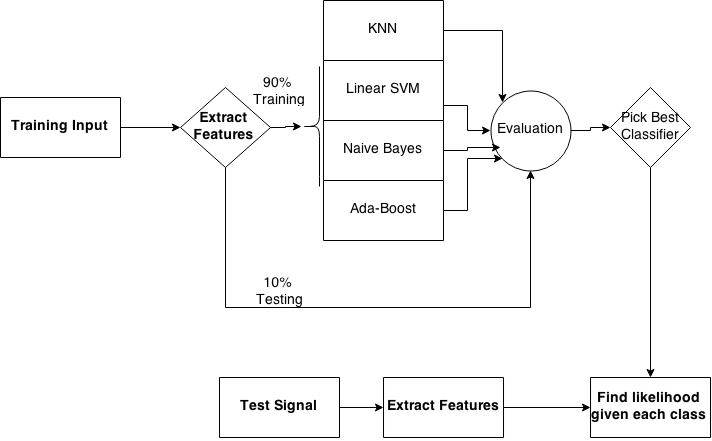
\includegraphics[width=8.3cm]{speech_class.jpg}}
\end{minipage}
\caption{Speech Classification)}
\label{fig:res}
\end{figure}
Now that we have our VAD and speech classifiers, we can easily assign labels to every analysis frames, e.g. no speech, class 1, class 1, class 2, etc. Given these labels, we can then find the location of each user at each frame from section III results and then reconstruct spatial audio using the techniques explained in section 2.1. 
\section{Results} 
We recorded a few video clips for which we attempted to reconstruct 3D audio from, the link is provided in [6]. For the first case, we simply tracked one person in a video frame, mapped his face location to HRTF angles and then reconstruct spatial audio using corresponding HRTF angles from the single channel audio input as was shown in figure 1. The resulting video is named as {\it $gobble\_cs598$.mp4} which as can also be found in [6]. For the second video, we recorded two speakers speaking, a snapshot was provided earlier in figure 2. We trained both speakers' facial and speech features beforehand as was discussed earlier in section III and IV and use that to find the face location. At every frame we detect and capture both speech and faces. Note that given our face model we already know where speakers are located at, so we simply classify each audio frame to one of three classes discussed in section IV. We can then create a spatial sound for the two users. \\ In general we were able to recreate a sound that was guided by speaker’s faces. We also included some example video clips where a piece of music was guided by the users face. This technology can be specifically useful in hearing aids. Imagine wearing google glass. You can capture faces using the glass and capture speech using your hearing aid. We can do tracking and classification either on the glass, offline or on the cloud and then feed the resulting information to the hearing aid to form beams toward the desired sound source and undo artifacts such as noise and reverberation in the room. \\ 
We use the same video with two speakers from last time, to perform multimodal speaker recognition. We can calculate the recognition of each speaker using equation 2. We, however, did not try to estimate $w's$ from the environment. We used values from $1$ to $10$ for $w$'s, where $1$ put more focus on the face classifier and 10, more weight on the speech classifier. We then evaluate the $P(user)_{k=1}^K$ over all video frames for all 10 values of $w$. We can then create a matrix of likelihoods as the one shown below.
\begin{align}P(user) = \begin{bmatrix}
p_{1,1}&\dots& p{1,10}\\
\vdots &\ddots &\vdots\\
p_{k,1}&\dots&p(k,10)
\end{bmatrix}\end{align}
We then look for a value of $w$ that maximizes the user classification at most frames, that is, 
\begin{align}
w_{max} = argmax_w(P(user)_{k=1}^K \&_ {w=1}^{10})
\end{align}
Where $K$ is the number of frames. 
For our video, it turned out that the value of $w$ is $4$. This means that the multimodal classifier is putting more weight on the face classifier. This makes sense since the face classifier was able to achieve higher accuracy than the speech classifier. 
\section{FUTURE WORK}
One of the assumptions made in section II was that speakers do not talk at the same time. One can the apply source separation techniques [7] on the input signals first based on the number of speakers in the room, and then follow the same procedure on section IV to classify each speaker into their corresponding classes while separating each source. \\

Another future enhancement is the ability to spatialize sounds other than speech in a desired video clip. A simple, but exhaustive way of doing this is to learn features for different objects and sounds as well. This will also require an even more exhaustive search of detecting and recognizing objects in defined blocks for every video frames. This work, however, could be useful for entertainment application, such as in movies and video games. Based on the key objects in the movie, one can learn a big database of sounds they make and their shape, and then reconstruct 3D audio throughout the whole clip, which might take hours or even days. \\

One can also use this project and apply it to teleconferencing applications as well. If you have a room full of stationary speakers, you can easily learn their facial and speech features by recording one of the sessions. One can then use the tracking procedure discussed in section III to locate each speaker and use the techniques explained in section IV to label the signal as well. That way if the conference room is equipped with microphone arrays, one can use this information to form the beam at the current speaker to enhance speech intelligibility. Note that in teleconferencing, we need to be able to do this in real time. There are assumptions that we can make to speed things up. For example, users are probably not moving around the room, so one only needs to locate them one time. After that, we only need to speech classification and labeling the signal where even assumption can be made given the application to simplify and speech up the process for real-time scenarios. \\ 

There are other possibilities for the future of this project. For example, is it possible to learn a relationship between speech and facial features using unsupervised methods? Earlier in figure 8 and 11 we depicted the facial and speech features for two and three classes respectively. We can use clustering methods to classify each group of features together, e.g. K-Means, GMM clustering or even better time series clustering such as Hidden Markov Models (HMM). One obvious disadvantages of clustering is obviously not having access to the labels of each class. For both 3D audio and speaker recognition, we need to have labels at each frame of analysis, e.g. given my speech signal, where is the user? Or given the speech and face likelihoods, who is the most likely speaker? We think there might be a relationship between facial features and its corresponding speech features at every frame. If such correlation exists between the two, one can find one's face just by analyzing the speech signals. \\

One last application that we can think of is to be able to perform supervised source separation. Since we already have a dictionary of Eigen faces and speeches for every user, we can simply scan the whole video frames and signals to extract ones face and speech by finding the best match between the signals and the corresponding Eigen values. This idea of unconstrained source separation has already been extensively investigated on video content analysis and sound recognitions in [8]. 

\newpage
\section{REFERENCE}
\

[1] Choueiri, E , Optimal Crosstalk Cancellation for Binaural Audio with Two Loudspeakers , Princeton University 

\centerline{}

[2] Binaural Recording. Wiki 100k. Princeton University.

\centerline{}

[3] Friedman, Michael. "Capturing spatial audio from arbitrary microphone arrays for binaural reproduction." (2014).

\centerline{}

[4] Gardner, Bill. "HRTF Measurements of a KEMAR Dummy-Head Microphone." HRTF Measurements of a KEMAR Dummy-Head Microphone. 

\centerline{}

[5] "Documentation." Face Detection and Tracking Using CAMShift. Web. 14 Dec. 2014. 

\centerline{}

[6] Recorded Videos. (https://www.dropbox.com/sh/
s16c6lrx9tay065/AADZpsofFS4ANiRzpQA8fHPca?dl=0)

\centerline{}

[7] Bryan, Nick J. "ISSE." Nick (Nicholas) J. Bryan. Stanford.

\centerline{}

[8] Paris Smaragdis. "Audio Demos." Audio Demos - Sound Recognition for Content Analysis
\end{document}



